\begin{frame}{Tests -- Set up}
8 Agents with 4 CPU(s), 8-16 GB of RAM, and 45 GB of Disk.

\begin{center}
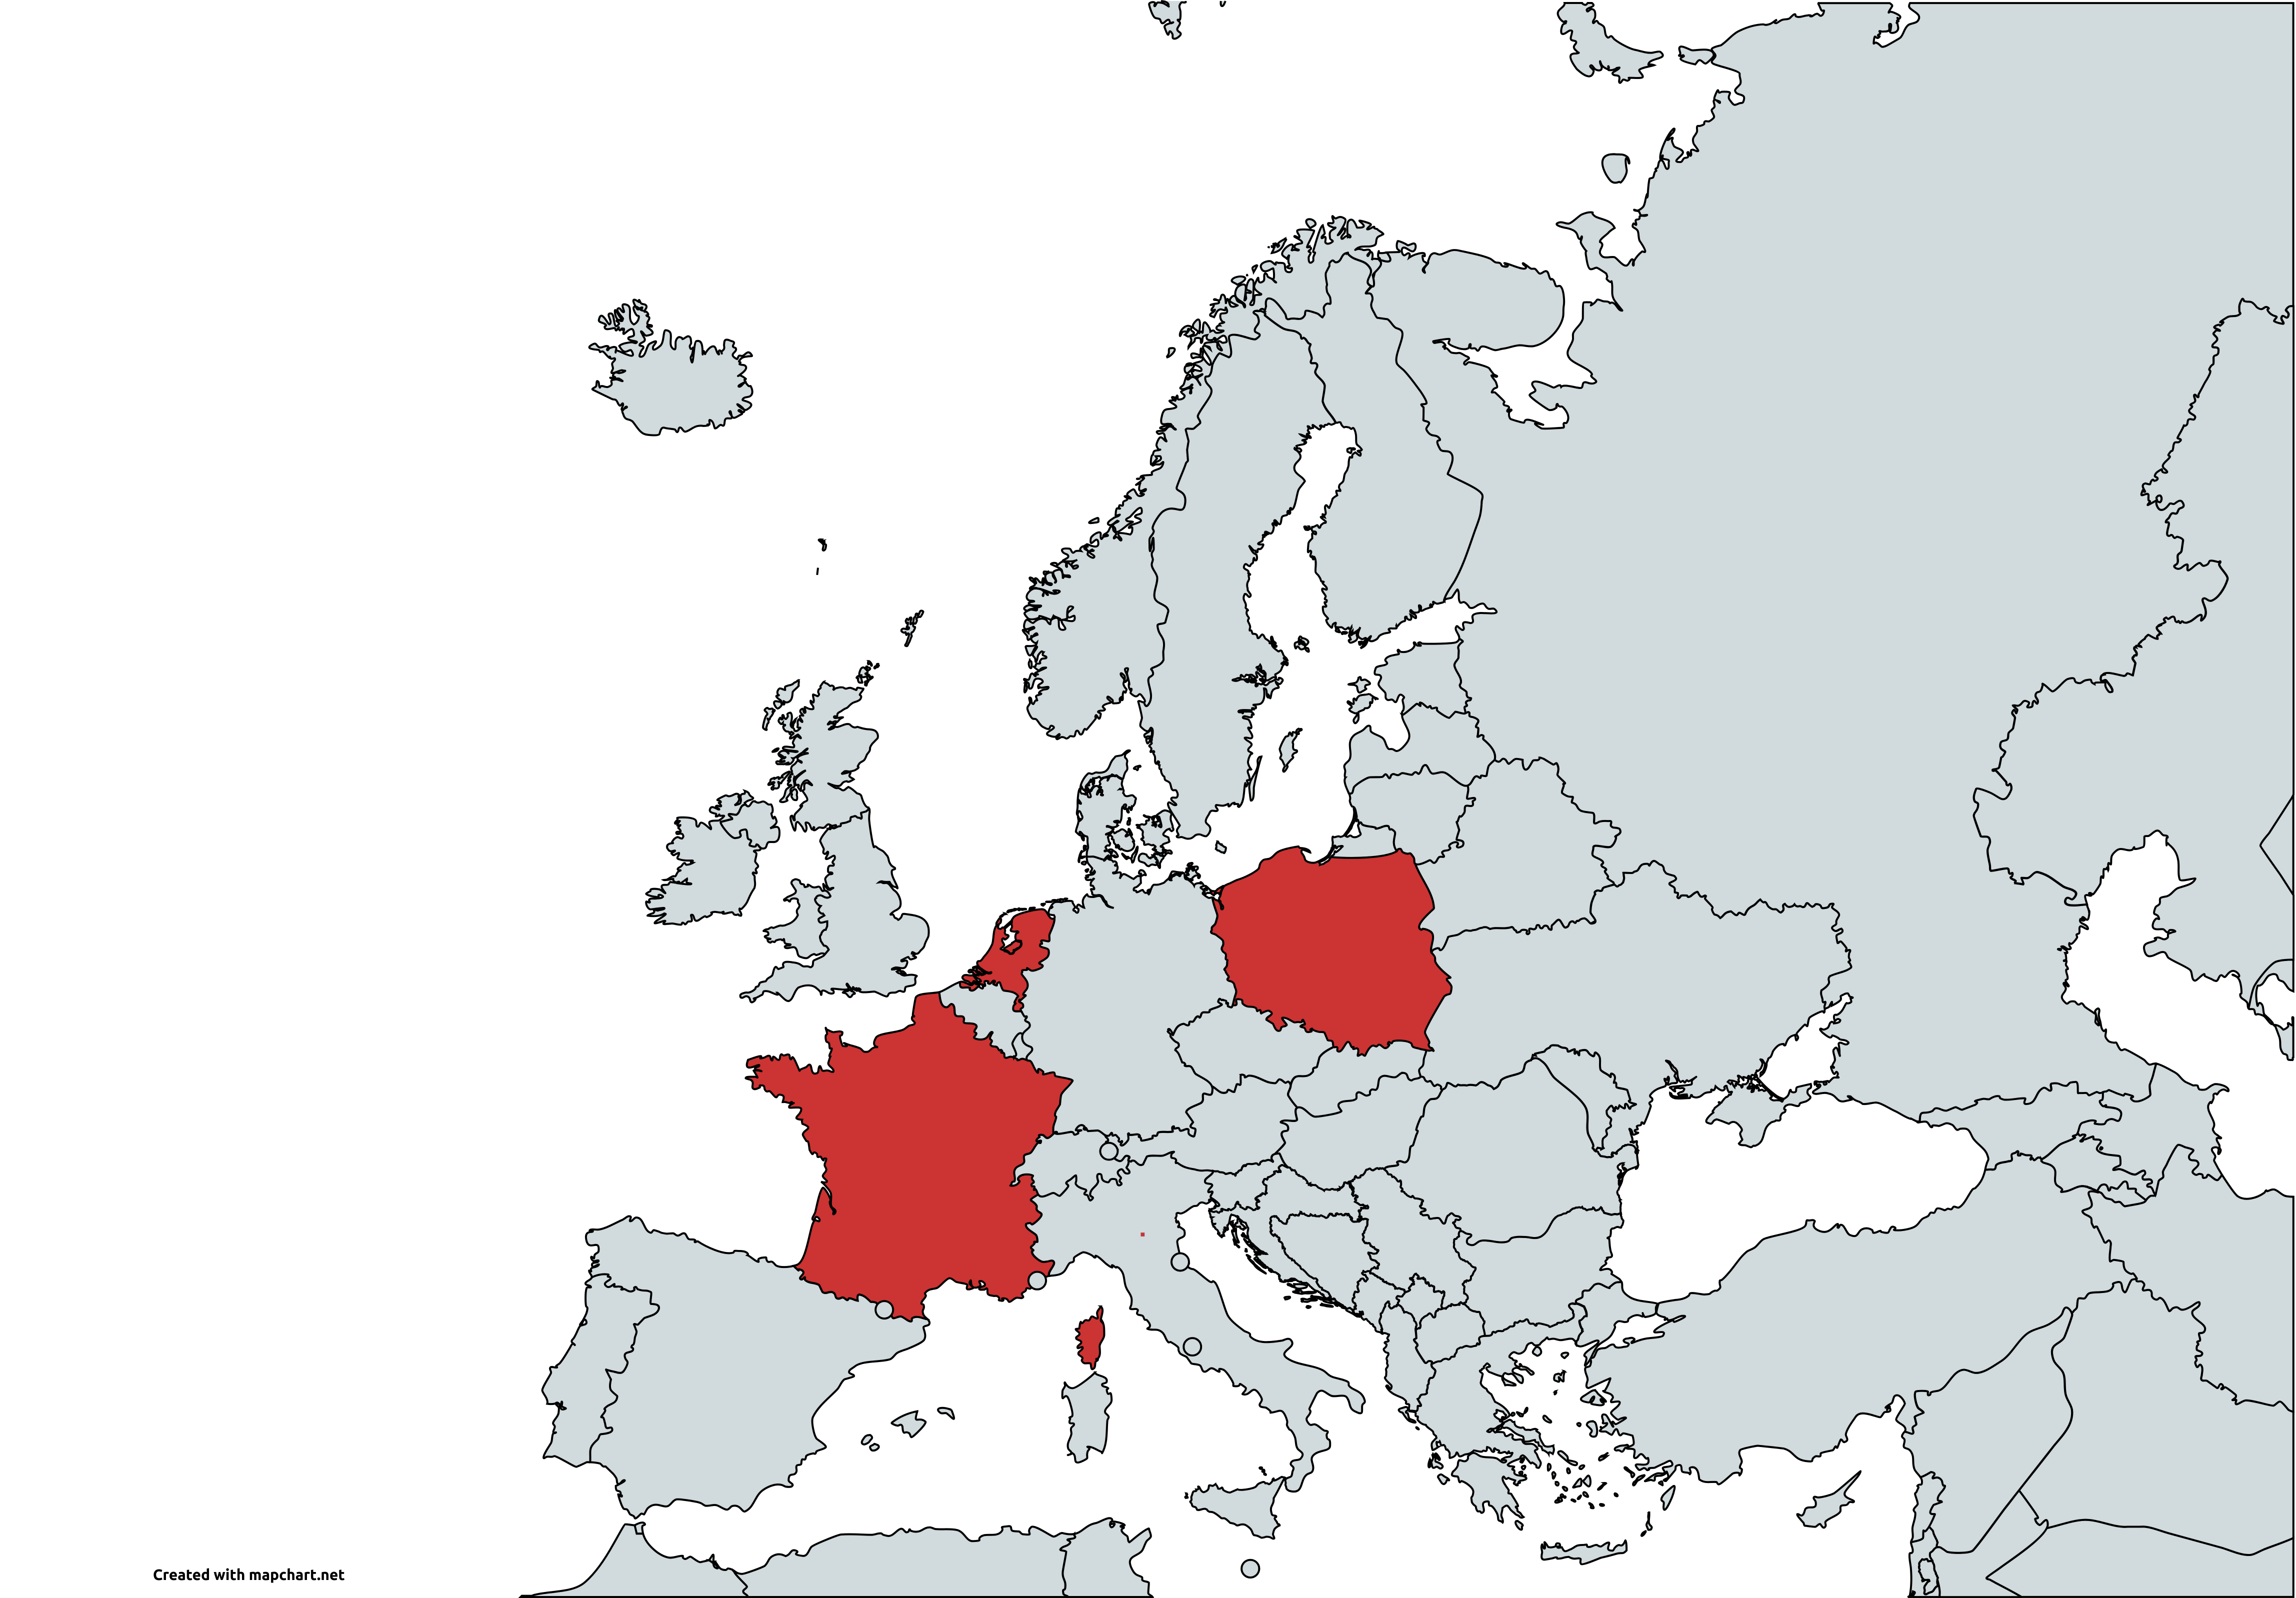
\includegraphics[width=0.5\linewidth]{static/map-chart.png}
\end{center}

For each test, we consider the number of online/offline agents and the file
    sizes and counts.

\end{frame}

\begin{frame}{Same dataset but different file size and count}

\begin{figure}
\centering
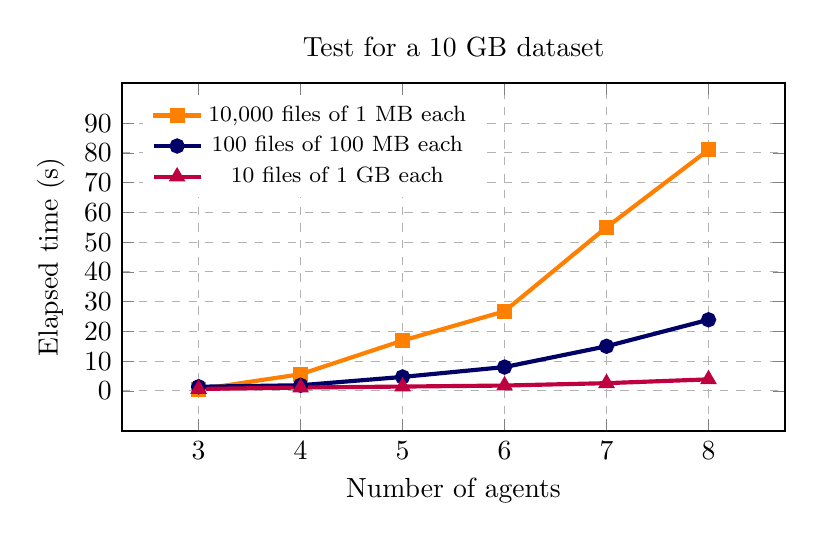
\begin{tikzpicture}
\begin{axis}[
    width=10cm, 
    height=6cm,
    xlabel={Number of agents},
    ylabel={Elapsed time (s)},
    xmin=3, 
    xmax=8,
    ymin=0, 
    ymax=90, % Max y value is ~81.032
    xtick={3,4,5,6,7,8},
    ytick={0,10,20,30,40,50,60,70,80,90},
    grid=major,
    grid style={dashed,gray!60},
    thick,
    title={Test for a 10 GB dataset},
    enlargelimits=0.15,
    legend pos=north west,
    legend style={draw=none, font=\footnotesize},
    % Option to show coordinates near the points for 10x1GB (optional, can be removed)
    % nodes near coords,
    % every node near coord/.append style={font=\tiny, anchor=south, yshift=2pt},
    % point meta=explicit symbolic
]

% 10,000 files of 1 MB each (Orange)
\addplot[color=orange, mark=square*, line width=1.5pt] coordinates {
    (3,0.4685) 
    (4,5.577) 
    (5,16.902) 
    (6,26.747) 
    (7,54.986) 
    (8,81.032) 
};
\addlegendentry{10,000 files of 1 MB each}

% 100 files of 100 MB each (Blue)
\addplot[color=blue!40!black, mark=*, line width=1.5pt] coordinates {
    (3,1.373) 
    (4,1.875) 
    (5,4.671) 
    (6,7.985) 
    (7,14.978) 
    (8,23.892) 
};
\addlegendentry{100 files of 100 MB each}


% 10 files of 1 GB each (Purple)
\addplot[color=purple, mark=triangle*, line width=1.5pt] coordinates {
    (3,0.6166) 
    (4,1.105) 
    (5,1.432) 
    (6,1.772) 
    (7,2.575) 
    (8,3.856) 
};
\addlegendentry{10 files of 1 GB each}

\end{axis}
\end{tikzpicture}
\end{figure}

\end{frame}

\begin{frame}{Test with offline agents}

\begin{figure}
\centering
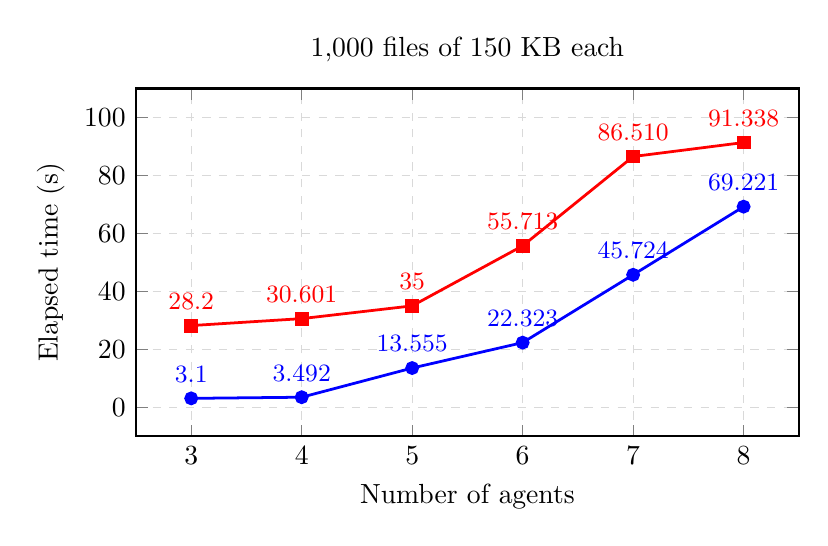
\begin{tikzpicture}
\begin{axis}[
    width=10cm, height=6cm,
    xlabel={Number of agents},
    ylabel={Elapsed time (s)},
    xmin=3, xmax=8,
    ymin=0, ymax=100,
    xtick={3,4,5,6,7,8},
    ytick={0,20,40,60,80,100},
    grid=major,
    grid style={dashed,gray!30},
    thick,
    title={1,000 files of 150 KB each},
    enlargelimits=0.1,
    clip=false,
    nodes near coords,
    every node near coord/.append style={font=\small, anchor=south, yshift=2pt},
    point meta=explicit symbolic
]

% Online agents
\addplot[color=blue, mark=*, line width=1pt] coordinates {
    (3,3.1) [3.1]
    (4,3.492) [3.492]
    (5,13.555) [13.555]
    (6,22.323) [22.323]
    (7,45.724) [45.724]
    (8,69.221) [69.221]
};

% Offline agents
\addplot[color=red, mark=square*, line width=1pt] coordinates {
    (3,28.2) [28.2]
    (4,30.601) [30.601]
    (5,35) [35]
    (6,55.713) [55.713]
    (7,86.510) [86.510]
    (8,91.338) [91.338]
};

\end{axis}
\end{tikzpicture}
\end{figure}

\end{frame}

\begin{frame}{Test with very large number of tiny files}

\begin{figure}
\centering
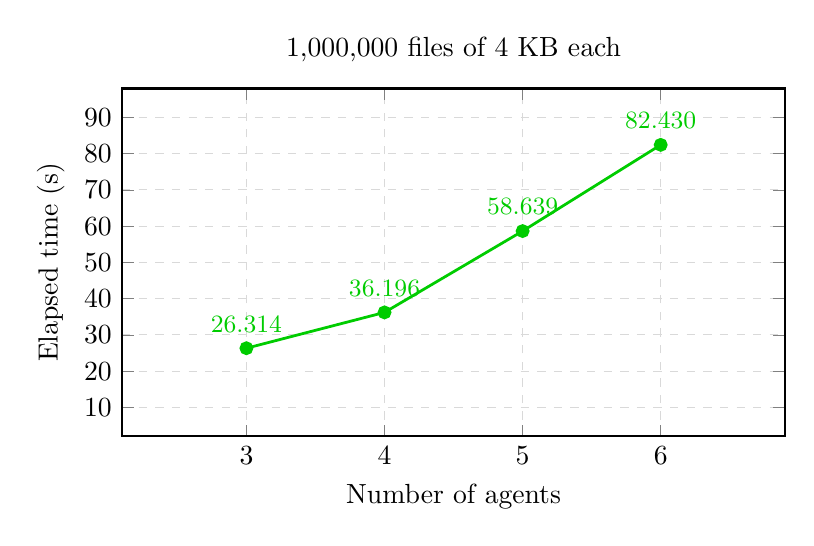
\begin{tikzpicture}
\begin{axis}[
    width=10cm, height=6cm,
    xlabel={Number of agents},
    ylabel={Elapsed time (s)},
    xmin=2.5, xmax=6.5,
    ymin=10, ymax=90,
    xtick={3,4,5,6},
    ytick={0,10,20,30,40,50,60,70,80,90,100},
    grid=major,
    grid style={dashed,gray!30},
    thick,
    title={1,000,000 files of 4 KB each},
    enlargelimits=0.1,
    clip=false,
    nodes near coords,
    every node near coord/.append style={font=\small, anchor=south, yshift=2pt},
    point meta=explicit symbolic
]

\addplot[color=green!80!black, mark=*, line width=1pt] coordinates {
    (3,26.314) [26.314]
    (4,36.196) [36.196]
    (5,58.639) [58.639]
    (6,82.430) [82.430]
};
\end{axis}
\end{tikzpicture}
\end{figure}

\end{frame}

\begin{frame}{Results}
\begin{itemize}
\item Scenarios with many small files amplify the cost of synchronization and consensus.
\item Verification time increases with the number of agents and files.
\item Confirmed the correctness and resilience of the approach under different scenarios and network conditions.
\end{itemize}
\end{frame}

\begin{frame}{Conclusion}

By combining Merkle trees, Raft consensus, and Reed-Solomon codes, we built a scalable and fault-tolerant protocol for distributed data integrity verification without relying on full file scans or constant node availability.

\vspace{2cm}
\centering
Thank you!
\end{frame}

